\chapter{Benutzerschnittstellen}

\section{Komponenten und Layouting}

Die Benutzerschnittstellen in Android sind hierarchisch aufgebaut und bestehen aus \texttt{ViewGroups} (Behälter für Views und andere ViewGroups) und \texttt{Views} (Widgets). Das Layout lässt sich entweder statisch in XML definieren oder dynamisch in Java. Normalerweise wird XML verwendet um ein Layout zu definieren. Nachfolgend werden einige Layouts beschrieben:
\begin{description}
	\item[LinearLayout:] Reiht Elemente neben-/untereinander auf. Kann geschachtelt werden, um Zeilen/Spalten zu formen. Mit dem Parameter \texttt{gravity} kann z.B. festgelegt werden wo es ein Objekt hinziehen soll.
	\item[RelativeLayout:] Ordnet Elemente entsprechend den zwischen ihnen definierten Relationen an (z.B. A neben B). Wenn man z.B. deklariert, dass ''A rechts von B'' und ''B rechts von A'' sein muss wird eine Exception geworfen (zyklische Abhängigkeit).
	\item[ScrollView:] Spezielle ViewGroup, die (vertikales) Scrolling bei zu grossen Layouts erlaubt (kann nur ein Kind haben).
\end{description}
Pixel-Angaben können auf drei verschiedene Arten gemacht werden. Dabei wird typischerweise \emph{dp} verwendet.
\begin{description}
	\item[dp (Density-independent Pixels):] Die Einheit ist relativ zu einem 160 dpi Bildschirm wo 1dp ungefähr 1px entspricht. Dadurch bleiben die Abmessungen über unterschiedliche Geräte im Verhältnis gleich.
	\item[sp (Scale-independent Pixels):] Die gleiche Einheit wie dp. Es wird aber zusätzlich noch die Schriftgrösse welcher der Benutzer eingestellt hat berücksichtigt. Sollte für Schriften verwendet werden.
	\item[px (Pixels):] Diese Einheit entspricht einem Pixel auf dem Bildschirm. Sollte nicht verwendet werden, weil die Darstellung über verschiedenen Geräte nicht einheitlich ist.
\end{description}

\section{Ressourcen, Konfigurationen \& Internationalisierung}

Ressourcen sind alle Nicht-Java Teile einer Applikation (z.B. Strings, Bilder, Layouts usw.). Ressourcen können aus einer XML-Datei z.B. mit einem \texttt{@color} referenziert werden. Im Code werden die Ressourcen über die automatisch generierte R-Klasse referenziert (z.B. \texttt{R.layout.activity\_main}). Es ist auch möglich spezifische Ressourcen zu definieren z.B. für die Internationalisierung oder für Bilder unterschiedlicher Auflösungen.
Alle Ressourcen werden im Verzeichnis \texttt{res/} abgelegt. In diesem Verzeichnis sind Default-Verzeichnisse für die verschiedenen Ressourcentypen (z.B. layout, values) angelegt. Spezifische Ressourcen legt man an indem man die Default-Verzeichnisse kopiert und mit einem Suffix ergänzt (z.B. values wird zu values-de für eine deutsche Übersetzung).

\section{UI Event Handling}

Jedes View-Element hat eine entsprechende Java-Klasse. Die Views werden im Code mit einer ID über die R-Klasse identifiziert, welche im XML definiert wurde. Für das Event Handling wird das Observer-Pattern verwendet, welches schon aus der Java-Welt bekannt ist (Listener für entsprechenden Event bei View registrieren). Abbildung \ref{fig:event-java} zeigt wie eine Button-ID im layout.xml definiert wird und der entsprechende Listener im Code registriert wird.
\begin{figure}
	\centering
	\begin{subfigure}[b]{0.48\textwidth}
		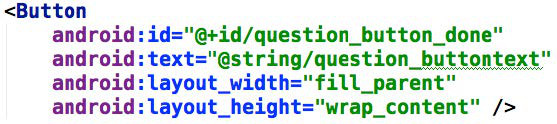
\includegraphics[width=\textwidth]{fig/event-java-id}
		\caption{\texttt{id} definieren}
	\end{subfigure}
	~
	\begin{subfigure}[b]{0.48\textwidth}
		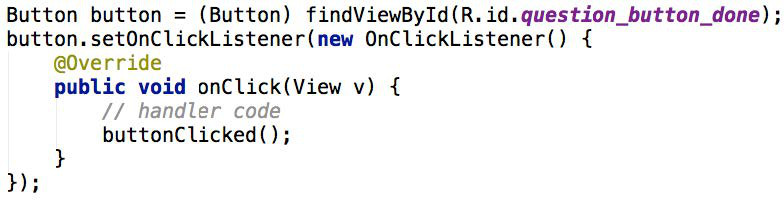
\includegraphics[width=\textwidth]{fig/event-java-listener}
		\caption{Button über \texttt{R}-Klasse holen}
	\end{subfigure}
	\caption{Eventhandler Java}
	\label{fig:event-java}
\end{figure}
Es ist auch möglich direkt im XML eine Methode als Listener zu registrieren (Abbildung \ref{fig:event-xml}).
\begin{figure}
	\centering
	\begin{subfigure}[b]{0.48\textwidth}
		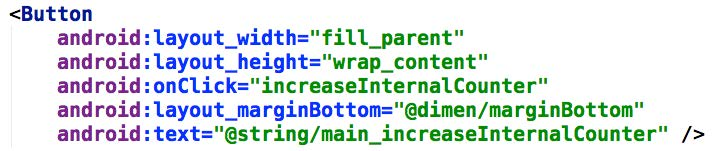
\includegraphics[width=\textwidth]{fig/event-xml-onclick}
		\caption{\texttt{onClick} definieren}
	\end{subfigure}
	~
	\begin{subfigure}[b]{0.48\textwidth}
		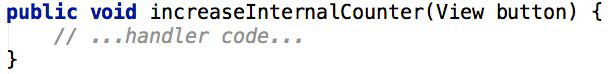
\includegraphics[width=\textwidth]{fig/event-xml-method}
		\caption{Aufgerufene Methode}
	\end{subfigure}
	\caption{Eventhandler XML}
	\label{fig:event-xml}
\end{figure}

\section{Options-Menu}

Android-Apps können in der Action-Bar rechts oben ein Menu mit Optionen pro Activity anbieten (seit Android 3 kein HW-Button mehr nötig). Das Menu wird in der Activity-Methode \texttt{onCreateOptionsMenu(Menu menu)} erzeugt. Bei einem Klick auf einen Menu-Eintrag wird \\ \texttt{onOptionsItemSelected(MenuItem item)} aufgerufen. Für die Erzeugung sind folgende Schritte notwendig:
\begin{enumerate}
	\item Ordner \texttt{res/menu} mit .xml-Datei anlegen (Dateiname z.B. main\_menu.xml)
	\item Menu und Items in XML definieren
	\item Menu ''aufblasen'' mit \texttt{MenuInflater}
\end{enumerate}
Abbildung \ref{fig:option-menu} zeigt den gesamten Ablauf nochmals als Code-Beispiel.
\begin{figure}
	\centering
	\begin{subfigure}[b]{0.48\textwidth}
		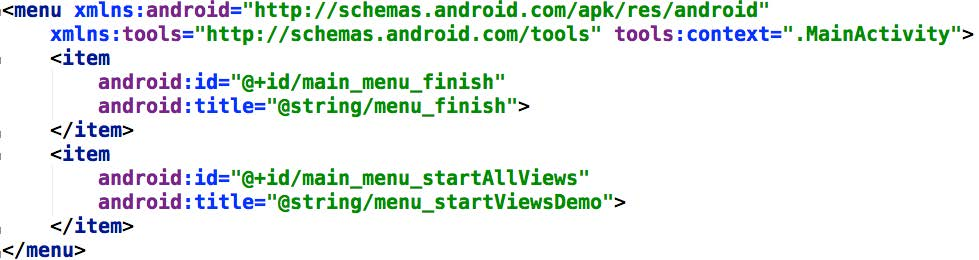
\includegraphics[width=\textwidth]{fig/option-menu-xml}
		\caption{Option Menu in XML}
	\end{subfigure}
	~
	\begin{subfigure}[b]{0.48\textwidth}
		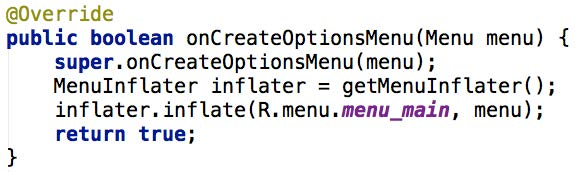
\includegraphics[width=\textwidth]{fig/option-menu-create}
		\caption{Menu aufblasen}
	\end{subfigure}
	~
	\begin{subfigure}[b]{0.48\textwidth}
		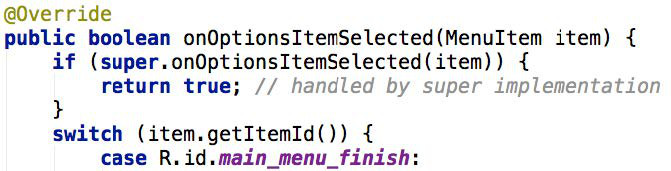
\includegraphics[width=\textwidth]{fig/option-menu-event}
		\caption{Option auswählen}
	\end{subfigure}
	\caption{Options-Menu}
	\label{fig:option-menu}
\end{figure}

\section{Adapter-Views}

Adapter sind die Verbindungen zwischen Datenquellen (String-Array, Bilder, Datenbank usw.) und der GUI. Der Adapter holt sich die Daten von der Datenquelle und beliefert den AdapterView. Die Daten werden in das benötigte Format transformiert und pro Datenelement wird eine (Sub-)View erzeugt. Ein Beispiel für einen Adapter ist der ArrayAdapter. Der ArrayAdapter nimmt als Datenquelle einen String-Array und erzeugt für jedes Datenelement einen TextView. Diese TextViews werden dann einem AdapterView übergeben.
Es gibt unter anderem folgende AdapterViews:
\begin{description}
	\item[Spinner:] Ein Spinner ist eine DropDown-List und wird für kurze Listen verwendet. Die Daten können entweder im XML mit dem Attribut \texttt{android:entries} oder mit der Methode \texttt{setAdapter} übergeben werden. Der Listener kann mit der Methode \texttt{setOnItemSelectedListener(...)} gesetzt werden.
	\item[ListView:] Stellt wie der Spinner Elemente als Liste dar und ist für die Verwendung mit langen Listen optimiert. Die Daten und Listener werden gleich wie beim Spinner definiert.
	\item[ListActivity:] Die ListActivity ist eine spezielle Activity welche die gleiche Darstellung wir die ListView hat, diese aber im full-screen anzeigt.
\end{description}

\section{Konfig.-Wechsel \& temporäre Datenspeicherung}

Bei jedem Konfigurationswechsel wird die aktuelle Activity zerstört und neu aufgebaut (z.B. Wechsel der Bildschirmorientierung). Dabei werden alle nicht sichtbareren Zustände (z.B. Instanzvariablen) verloren. Deshalb sollten Activities keine Zustände haben sondern diese in Services ausgelagert werden. Schlüssel-Werte-Paare können auch kurzfristig in-memory gespeichert werden. Abbildung \ref{fig:instance-state} zeigt ein Code-Beispiel um das Verhalten umzusetzen.
\begin{figure}
	\centering
	\begin{subfigure}[b]{0.48\textwidth}
		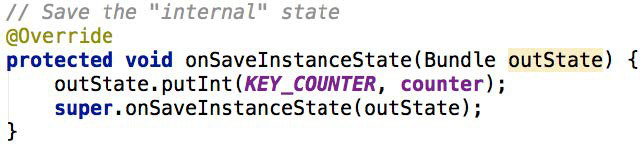
\includegraphics[width=\textwidth]{fig/save-instance}
		\caption{Daten speichern}
	\end{subfigure}
	~
	\begin{subfigure}[b]{0.48\textwidth}
		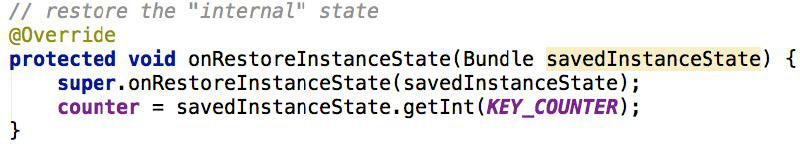
\includegraphics[width=\textwidth]{fig/restore-instance}
		\caption{Daten laden}
	\end{subfigure}
	\caption{Temporäre Datenspeicherung}
	\label{fig:instance-state}
\end{figure}

\section{Rückmeldung an den Benutzer}

\subsection{Toast}

Ein Toast ist eine kurze Rückmeldung (Popup) an Benutzer (keine Interaktion möglich). Toats lassen sich sehr einfach erstellen, können aber auch leicht übersehen werden. Abbildung \ref{fig:toast} zeigt wie ein Toast erstellt wird.
\begin{figure}
\centering
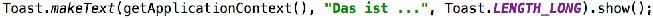
\includegraphics[width=\linewidth]{fig/toast}
\caption{Toast}
\label{fig:toast}
\end{figure}

\subsection{Alert-Dialog}

Ein Alert-Dialog ist ein Fenster mit Rückmeldung an den Benutzer. Der Benutzer kann mit dem Fenster interagieren und die Darstellung kann individuell (z.B. ListView für Liste von Items) angepasst werden. Abbildung \ref{fig:alert-dialog} zeigt die etwas mühsame Erstellung eines Alert-Dialog.

\begin{figure}
\centering
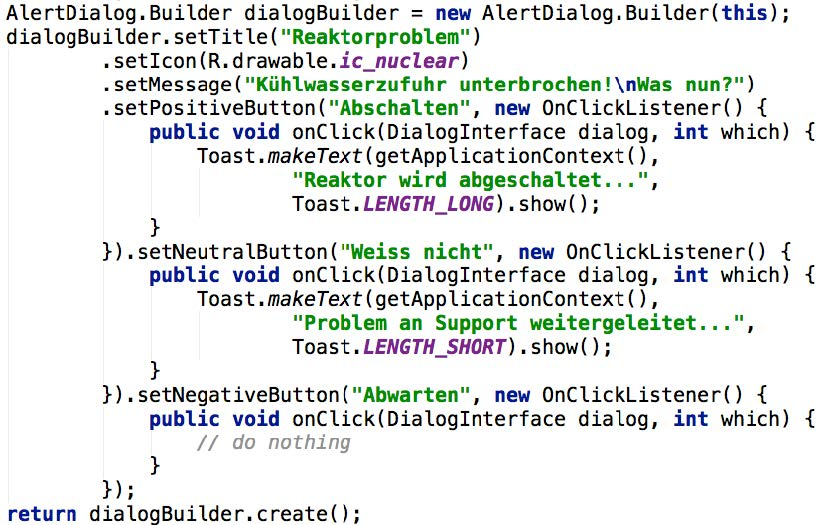
\includegraphics[width=0.7\linewidth]{fig/alert-dialog}
\caption{Alert Dialog}
\label{fig:alert-dialog}
\end{figure}

\subsection{Notifications}

Notifications sind persistente Nachrichten welche in der Status-Bar angezeigt werden. Bei Auswahl erfolgt Aufruf einer definierten Activity. Die Erstellung einer Notification ist relativ komplex, darum wird kein Code-Beispiel gegeben.